\section*{静电场}

\subsubsection*{一. 选择题}

1. 一均匀带电球面,电荷面密度为$\sigma$,球面内电场强度处处为零,球面上面元$\d S$带有$\sigma\d S$的电荷,该电荷在球面内各点产生的电场强度\fbox{处处不为零}.

2. 下列说法中正确的是\ul{场强可由$\vec{E}=\vec{F}/q$定出,其中$q$为试验电荷可负可正,$\vec{F}$为试验电荷所受的电场力}.

4. 将一个试验电荷$q_0$(正电荷)放在带有负电荷的大导体附近$P$点处(如图),测得它所受的力为$F$.若考虑到电荷$q_0$不是足够小,则\ul{$F/q_0$比$P$点处原先的场强数值小}.

图4.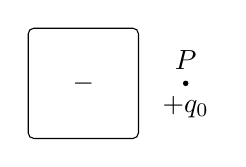
\begin{tikzpicture}
\draw[rounded corners=2pt] (0,0) rectangle (1.4,1.4);
\draw (0.7,0.7) node {$-$};
\fill (2,0.7) circle (1pt);
\draw (2,1) node {$P$};
\draw (2,0.4) node {$+q_0$};
\end{tikzpicture}
图7.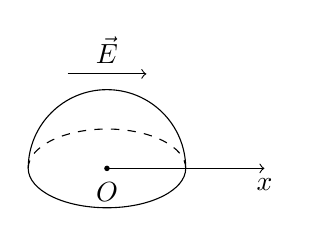
\begin{tikzpicture}
\draw (0,0) arc [start angle=0, end angle=180, x radius=1, y radius=1];
\draw[dashed] (0,0) arc [start angle=0, end angle=180, x radius=1, y radius=0.5];
\draw (0,0) arc [start angle=360, end angle=180, x radius=1, y radius=0.5];
\draw[->] (-1.5,1.2) -- (-0.5,1.2);
\draw (-1,1.5) node {$\vec E$};
\fill (-1,0) circle (1pt);
\draw (-1,-0.3) node {$O$};
\draw[->] (-1,0) -- (1,0);
\draw (1,-0.2) node {$x$};
\end{tikzpicture}
图8.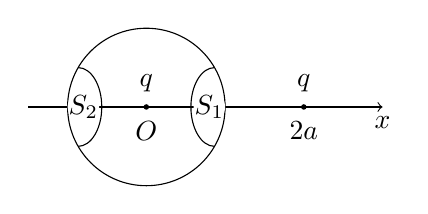
\begin{tikzpicture}
\draw (0,0) circle (1);
\fill (0,0) circle (1pt);
\draw (0,0.3) node {$q$};
\draw (0,-0.3) node {$O$};
\draw[->] (-1.5,0) -- (3,0);
\draw (3,-0.2) node {$x$};
\fill (2,0) circle (1pt);
\draw (2,0.3) node {$q$};
\draw (2,-0.3) node {$2a$};
\draw (30:1) arc [start angle=90, delta angle=180, y radius=0.5, x radius=0.3];
\fill[white] (0.8,0) circle (0.2);
\draw (0.8,0) node {$S_1$};
\draw (210:1) arc [start angle=270, delta angle=180, y radius=0.5, x radius=0.3];
\fill[white] (-0.8,0) circle (0.2);
\draw (-0.8,0) node {$S_2$};
\end{tikzpicture}

7. 一电场强度为$\vec E$的均匀电场,$\vec E$的方向沿$x$轴正方向,如图,则通过图中一半径为$R$的半球面的电场强度通量为\fbox{0}.

8. 有两个电荷都是$+q$的点电荷,相距为$2a$.今以左边的点电荷所在处为球心,以$a$为半径作一球形高斯面.在球面上取两块相等的小面积$S_1$和$S_2$,其位置如图所示.设通过$S_1$和$S_2$的电场强度通量分别为$\varPhi_1$和$\varPhi_2$,通过整个球面的电场强度通量为$\varPhi_S$,则\fbox{$\varPhi_1<\varPhi_2, \varPhi_S=q/\eo $}.

9. 如图所示,一个电荷为$q$的点电荷位于立方体的$A$角上,则通过侧面$abcd$的电场强度通量等于\fbox{$\frac{q}{24\eo }$}.

图9.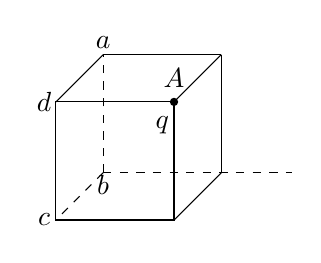
\begin{tikzpicture}[scale=1.5]
\draw (0,0) rectangle (1,1);
\draw[dashed] (0.4,0.4) -- (0.4,1.4);
\draw[dashed] (0.4,0.4) -- (2,0.4);
\draw[dashed] (0.4,0.4) -- (0,0);
\draw (0,1) -- (0.4,1.4);
\draw (1,1) -- (1.4,1.4);
\draw (1,0) -- (1.4,0.4);
\draw (0.4,1.4) -- (1.4,1.4);
\draw (1.4,0.4) -- (1.4,1.4);
\draw (-0.1,0) node {$c$};
\draw (-0.1,1) node {$d$};
\draw (0.4,1.5) node {$a$};
\draw (0.4,0.3) node {$b$};
\fill (1,1) circle (1pt);
\draw (1,1.2) node {$A$};
\draw (0.9,0.8) node {$q$};
\end{tikzpicture}
图10.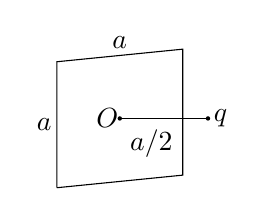
\begin{tikzpicture}[scale=0.8]
\draw (-1,-1) -- (-1,1) -- (1,1.2) -- (1,-0.8) -- (-1,-1);
\fill (0,0.1) circle (1pt);
\draw (-0.2,0.1) node {$O$};
\draw (0,0.1) -- (1.4,0.1);
\draw (0.5,-0.3) node {$a/2$};
\draw (-1.2,0) node {$a$};
\draw (0,1.3) node {$a$};
\fill (1.4,0.1) circle (1pt);
\draw (1.6,0.1) node {$q$};
\end{tikzpicture}
图16.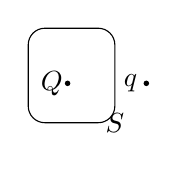
\begin{tikzpicture}
\draw[rounded corners=6pt] (0,0) rectangle (1.1,1.2);
\draw (1.1,0) node {$S$};
\fill (0.5,0.5) circle (1pt);
\draw (0.3,0.5) node {$Q$};
\fill (1.5,0.5) circle (1pt);
\draw (1.3,0.5) node {$q$};
\end{tikzpicture}

10. 有一边长为$a$的正方形平面,在其中垂线上距中心$O$点$a/2$处,有一电荷为$q$的正点电荷,如图所示,则通过该平面的电场强度通量为\fbox{$\frac{q}{6\eo }$}.

11. 高斯定理$\oint_S\vec E\cdot\d\vec S=\int_V\rho\d V/\eo $ \ul{适用于任何静电场}.

12. 关于高斯定理的理解有下面几种说法,其中正确的是\ul{如果高斯面内有静电荷,则通过高斯面的电场强度通量必不为零}.

15. 根据高斯定理的数学表达式$\oint_S\vec E\cdot\d\vec S=\sum q/\eo $可知\ul{闭合面内的电荷代数和为零时,闭合面上各点场强不一定处处为零}.

16. 点电荷$Q$被曲面$S$所包围,从无限远处引入另一点电荷$q$至曲面外一点,如图所示,则引入前后\ul{曲面$S$的电场强度通量不变,曲面上各点场强变化}.

17. 半径为$R$的均匀带电球体的静电场中各点的电场强度大小$E$与距球心距离$r$的关系曲线为\fbox{(B)}.

图17.(B)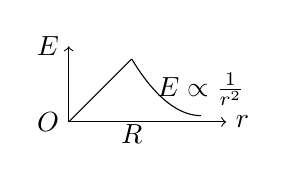
\begin{tikzpicture}[scale=0.8]
\draw (0,0) node[left] {$O$};
\draw[->] (0,0) -- (2.5,0) node[right] {$r$};
\draw[->] (0,0) -- (0,1.2) node[left] {$E$};
\draw (1,-0.2) node {$R$};
\draw (0,0) -- (1,1);
\draw (1,1) parabola[bend at end] (2.1,0.1) node[above] {$E\propto\D\frac{1}{r^2}$};
% \draw[dashed] (1,0) -- (1,1);
\end{tikzpicture}
图18.(B)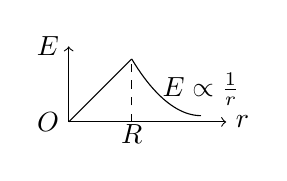
\begin{tikzpicture}[scale=0.8]
\draw (0,0) node[left] {$O$};
\draw[->] (0,0) -- (2.5,0) node[right] {$r$};
\draw[->] (0,0) -- (0,1.2) node[left] {$E$};
\draw (1,-0.2) node {$R$};
\draw (0,0) -- (1,1);
\draw (1,1) parabola[bend at end] (2.1,0.1) node[above] {$E\propto\D\frac{1}{r}$};
\draw[dashed] (1,0) -- (1,1);
\end{tikzpicture}

18. 半径为$R$的“无限长”均匀带电圆柱体的静电场中各点的电场强度大小$E$与距轴线距离$r$的关系曲线为\fbox{(B)}.

23. 有$N$个电荷均为$q$的点电荷,以两种方式分布在相同半径的圆周上:一种是无规则的分布,另一种是均匀分布.比较这两种情况下在过圆心$O$并垂直于圆平面的$z$轴上任一点$P$(如图所示)的场强与电势,则有\ul{场强分量$E_z$相等,电势相等}.

24. 静电场中某点电势的数值等于\ul{单位正电荷置于该点时具有的电势能}.

25. 关于静电场中某点电势值的正负,\ul{电势值的正负取决于电势零点的选取}.

26. 如图,在点电荷$q$的电场中,选取以$q$为中心、$R$为半径的球面上一点$P$处作电势零点,则与点电荷$q$距离为$r$的点$P'$电势为\fbox{$\frac{q}{4\pi\eo }(\frac{1}{r}-\frac{1}{R})$}.

图23.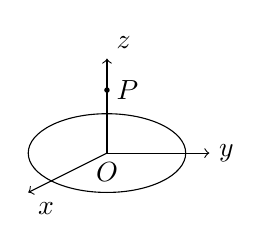
\begin{tikzpicture}
\draw (0,0) node[below] {$O$};
\draw[->] (0,0) -- (-1,-0.5) node[below right] {$x$};
\draw[->] (0,0) -- (1.3,0) node[right] {$y$};
\draw[->] (0,0) -- (0,1.2) node[above right] {$z$};
\fill (0,0.8) circle(1pt) node[right] {$P$};
\draw (0,0) ellipse[x radius=1,y radius=0.5];
\end{tikzpicture}
图26.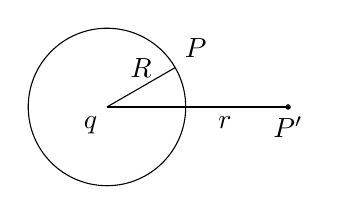
\begin{tikzpicture}
\draw (0,0) circle (1);
\draw (0,0) -- (30:1);
\draw (30:.5) node[above] {$R$};
\draw (30:1) node[above right] {$P$};
\draw (0,0) node[below left] {$q$};
\draw (0,0) -- (2.3,0);
\draw (1.5,0) node[below] {$r$};
\fill (2.3,0) circle (1pt);
\draw (2.3,0) node[below] {$P'$};
\end{tikzpicture}
图27.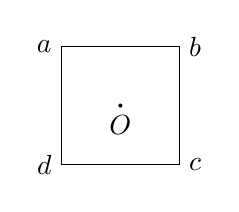
\begin{tikzpicture}[scale=1.5]
\draw (0,0) rectangle (1,1);
\draw (0,0) node[left] {$d$};
\draw (0,1) node[left] {$a$};
\draw (1,0) node[right] {$c$};
\draw (1,1) node[right] {$b$};
\fill (.5,.5) circle (.5pt) node[below] {$O$};
\end{tikzpicture}

27. 如图所示,边长为$l$的正方形,在其四个顶点上各放有等量的点电荷.若正方形中心$O$处的场强值和电势值都等于零,则\ul{顶点$a,c$处是正电荷,$b,d$处是负电荷}.

30. 如图所示,两个同心球壳.内球壳半径为$R_1$,均匀带有电荷$Q$;外球壳半径为$R_2$,壳的厚度忽略,原先不带电,但与地相连接.设地为电势零点,则在两球之间距离球心为$r$的点$P$处电场强度大小为\fbox{$E=\frac{Q}{4\pi\eo r^2}$},电势为\fbox{$U=\frac{Q}{4\pi\eo }(\frac{1}{r}-\frac{1}{R})$}.

图30.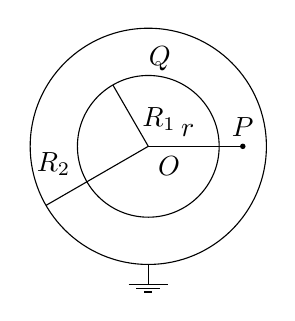
\begin{tikzpicture}[scale=0.5]
\draw (0,0) node[below right] {$O$};
\draw (0,0) circle (1.8);
\draw (0,0) circle (3);
\draw (0,0) -- (120:1.8);
\draw (120:0.8) node[right] {$R_1$};
\draw (80:1.7) node[above] {$Q$};
\draw (0,0) -- (210:3);
\draw (210:2) node[above left] {$R_2$};
\draw (0,0) -- (2.4,0);
\draw (1,0) node[above] {$r$};
\fill (2.4,0) circle (2pt);
\draw (2.4,0) node[above] {$P$};
\draw (0,-3) -- (0,-3.5);
\draw (-0.5,-3.5) -- (0.5,-3.5);
\draw (-0.3,-3.6) -- (0.3,-3.6);
\draw (-0.1,-3.7) -- (0.1,-3.7);
\end{tikzpicture}
图32.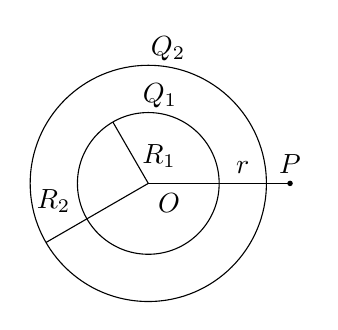
\begin{tikzpicture}[scale=0.5]
\draw (0,0) node[below right] {$O$};
\draw (0,0) circle (1.8);
\draw (0,0) circle (3);
\draw (0,0) -- (120:1.8);
\draw (120:0.8) node[right] {$R_1$};
\draw (80:1.7) node[above] {$Q_1$};
\draw (80:2.9) node[above] {$Q_2$};
\draw (0,0) -- (210:3);
\draw (210:2) node[above left] {$R_2$};
\draw (0,0) -- (3.6,0);
\draw (2.4,0) node[above] {$r$};
\fill (3.6,0) circle (2pt);
\draw (3.6,0) node[above] {$P$};
\end{tikzpicture}
图33.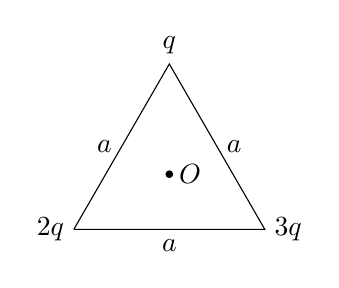
\begin{tikzpicture}[scale=1.4]
\draw (210:1) -- (90:1) -- (330:1) -- (210:1);
\fill (0,0) circle (1pt);
\draw (0,0) node[right] {$O$};
\draw (210:1) node[left] {$2q$};
\draw (90:1) node[above] {$q$};
\draw (330:1) node[right] {$3q$};
\draw (30:.5) node[right] {$a$};
\draw (150:.5) node[left] {$a$};
\draw (270:.5) node[below] {$a$};
\end{tikzpicture}

32. 如图所示,两个同心的均匀带电球面,内球面半径为$R_1$、带电荷$Q_1$,外球面半径为$R_2$、带电荷$Q_2$.设无穷远处为电势零点,则在外球面之外距离球心为$r$处的点$P$的电势$U$为\fbox{$\frac{Q_1+Q_2}{4\pi\eo r}$}.

33. 如图所示,边长为$a$的等边三角形的三个顶点上,分别放置着三个正的点电荷$q,2q,3q$.若将另一正点电荷$Q$从无穷远处移到三角形中心$O$处,外力所做的功为\fbox{$\frac{3\sqrt{3}qQ}{2\pi\eo a}$}.

34. 点电荷$-q$位于圆心$O$处,$A,B,C,D$为同一圆周上的四点,如图所示.现将一试验电荷从$A$点分别移动到$B,C,D$各点,则\ul{从$A$到各点,电场力做功相等}.

图34.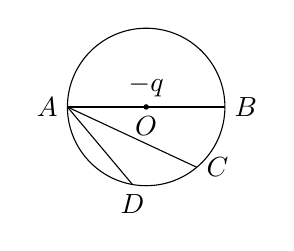
\begin{tikzpicture}
\draw (0,0) node[below] {$O$};
\draw (0,0) node[above] {$-q$};
\draw (0,0) circle (1);
\fill (0,0) circle (1pt);
\draw (-1,0) node[left] {$A$}
    -- (1,0) node[right] {$B$};
\draw (-1,0) -- (310:1) node[right] {$C$};
\draw (-1,0) -- (260:1) node[below] {$D$};
\end{tikzpicture}
图35.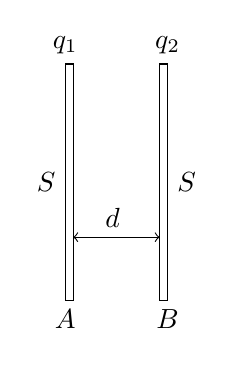
\begin{tikzpicture}
\draw (0,0) rectangle (.1,3);
\draw (1.2,0) rectangle (1.3,3);
\draw (0,1.5) node[left] {$S$};
\draw (0,3) node[above] {$q_1$};
\draw (0,0) node[below] {$A$};
\draw (1.3,1.5) node[right] {$S$};
\draw (1.3,0) node[below] {$B$};
\draw (1.3,3) node[above] {$q_2$};
\draw[<->] (0.1,0.8) -- (1.2,0.8);
\draw (0.6,0.8) node[above] {$d$};
\end{tikzpicture}
图36.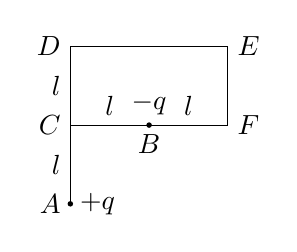
\begin{tikzpicture}
\draw (0,0) rectangle (2,1);
\draw (0,0) node[left] {$C$};
\draw (0,1) node[left] {$D$};
\draw (2,1) node[right] {$E$};
\draw (2,0) node[right] {$F$};
\draw (0,0) -- (0,-1) node[left] {$A$};
\fill (0,-1) circle (1pt) node[right] {$+q$};
\fill (1,0) circle (1pt);
\draw (1,0) node[below] {$B$};
\draw (1,0) node[above] {$-q$};
\draw (0,0.5) node[left] {$l$};
\draw (0,-0.5) node[left] {$l$};
\draw (0.5,0) node[above] {$l$};
\draw (1.5,0) node[above] {$l$};
\end{tikzpicture}

35. 两块面积均为$S$的金属平板$A$和$B$彼此平行放置,板间距离为$d$($d$远小于板的线度),设$A$板带有电荷$q_1$,$B$板带有电荷$q_2$,则$A,B$两板间的电势差$U_{AB}$为\fbox{$\frac{q_1-q_2}{2\eo S}d$}.

36. 如图所示,$CDEF$为一矩形,边长分别为$l$和$2l$.在$DC$延长线上$CA=l$处的$A$点有点电荷$+q$,在$CF$的中点$B$有点电荷$-q$,若使单位正电荷从$C$点沿$CDEF$径运动到$F$点,则电场力所做的功等于\fbox{$\frac{q}{4\pi\eo l}\cdot\frac{\sqrt5-1}{\sqrt5}$}.

37. 图中实线为某电场中的电场线,虚线表示等势(位)面,由图可以看出\ul{$E_A<E_B<E_C,$ $U_A>U_B>U_C$}.

图37.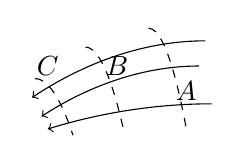
\begin{tikzpicture}[scale=0.8]
% \draw[help lines] (0,0) grid (3,2);
\draw[->] (3,0.4) parabola (0.4,0);
\draw[dashed] (2,1.6) parabola (2.6,0);
\draw (2.6,0.6) node {$A$};
\draw[->] (2.8,1) parabola (0.3,0.2);
\draw[dashed] (1,1.3) parabola (1.6,0);
\draw (1.5,1) node {$B$};
\draw[->] (2.9,1.4) parabola (0.15,0.5);
\draw[dashed] (0.2,0.8) parabola (0.8,-0.1);
\draw (0.4,1) node {$C$};
\end{tikzpicture}
图38.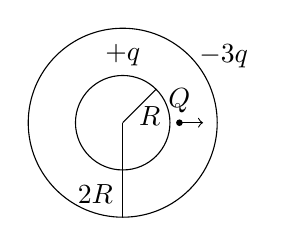
\begin{tikzpicture}[scale=0.6]
\draw (0,0) circle (1);
\draw (0,0) circle (2);
\draw (0,0) -- (45:1);
\draw (0,0) -- (270:2);
\draw (45:.2) node[right] {$R$};
\draw (270:1.5) node[left] {$2R$};
\fill (1.2,0) circle (2pt) node[above] {$Q$};
\draw[->] (1.2,0) -- (1.7,0);
\draw (90:1) node[above] {$+q$};
\draw (45:2) node[right] {$-3q$};
\end{tikzpicture}
图47.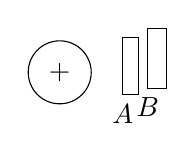
\begin{tikzpicture}[scale=0.4]
\draw (0,0) circle (1);
\draw (0,0) node {$+$};
\draw (2,-0.7) node[below] {$A$} rectangle (2.5,1.1);
\draw (2.8,-0.5) node[below] {$B$} rectangle (3.4,1.4);
\end{tikzpicture}
图48.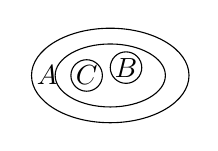
\begin{tikzpicture}
\draw (0,0) circle[x radius=1,y radius=0.6];
\draw (0,0) circle[x radius=0.7,y radius=0.4];
\draw (-0.3,0) node {$C$} circle (0.2);
\draw (0.2,0.1) node{$B$} circle (0.2);
\draw (-0.8,0) node {$A$};
\end{tikzpicture}

38. 如图所示,在真空中半径分别为$R$和$2R$的两个同心球面,其上分别均匀地带有电荷$+q$和$-3q$.今将一电荷为$+Q$的带电粒子从内球面处由静止释放,则该粒子到达外球面时的动能为\fbox{$\frac{Qq}{8\pi\eo R}$}.

47. 把$A,B$两块不带电的导体放在一带正电导体的电场中,如图所示.设无限远处为电势零点,$A$的电势为$U_A$,$B$的电势为$U_B$,则\fbox{$U_B<U_A$}.

48. 如图所示,一封闭的导体壳$A$内有两个导体$B$和$C$.$A,C$不带电,$B$带正电,则$A,B,C$三导体的电势关系是\fbox{$U_B>U_C>U_A$}.

52. 一个平行板电容器,充电后与电源断开,当用绝缘手柄将电容器两极板间距拉大,则两级板间的电势差\fbox{$U_{12}$增大},电场强度大小\fbox{$E$不变},电场能量\fbox{$W$增大}.

\subsubsection*{二. 填空题}

57. $A,B$为真空中两个平行的“无限大”的均匀带电平面,已知两平面间的电场强度大小为$E_0$,两平面外侧电场强度大小都为$E_0/3$,方向如图,则$A,B$两平面上的电荷面密度分别为$\sigma_A=$\fbox{$-\frac{2}{3}\eo E_0$},$\sigma_B=$\fbox{$\frac{4}{3}\eo E_0$}.

图57.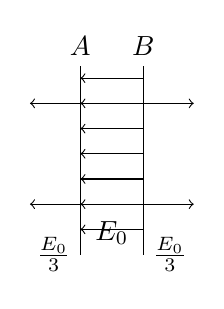
\begin{tikzpicture}[scale=0.8]
\draw (0,0) -- (0,3);
\draw (1,0) -- (1,3);
\draw (0,3) node[above] {$A$};
\draw (0,0) node[left] {$\frac{E_0}{3}$};
\draw (1,3) node[above] {$B$};
\draw (1,0) node[right] {$\frac{E_0}{3}$};
\draw (0.5,0) node[above] {$E_0$};
\draw[<-] (0,0.4) -- (1,0.4);
\draw[<-] (0,0.8) -- (1,0.8);
\draw[<->] (-0.8,0.8) -- (1.8,0.8);
\draw[<-] (0,1.2) -- (1,1.2);
\draw[<-] (0,1.6) -- (1,1.6);
\draw[<-] (0,2) -- (1,2);
\draw[<-] (0,2.4) -- (1,2.4);
\draw[<->] (-0.8,2.4) -- (1.8,2.4);
\draw[<-] (0,2.8) -- (1,2.8);
\end{tikzpicture}
图60.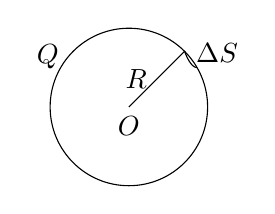
\begin{tikzpicture}
\draw (0,0) node[below] {$O$} circle (1);
\draw (0,0) -- (45:1);
\draw (45:.5) node[left] {$R$};
\draw (140:1) node[left] {$Q$};
\draw (45:1) parabola[bend at end] (30:1);
\draw (43:1) node[right] {$\Delta S$};
\end{tikzpicture}
图61.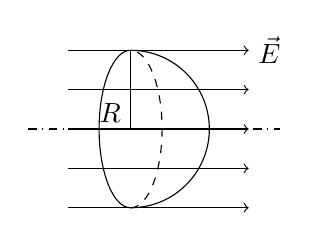
\begin{tikzpicture}
\draw (0.5,0) arc [start angle=270, delta angle=180, y radius=1, x radius=1];
\draw[dashed] (0.5,0) arc [start angle=270, delta angle=180, y radius=1, x radius=0.4];
\draw (0.5,2) arc [start angle=90, delta angle=180, y radius=1, x radius=0.4];
\draw (0.5,1) -- (0.5,2);
\draw (0.5,1.2) node[left] {$R$};
\draw[->] (-0.3,0) -- (2,0);
\draw[->] (-0.3,0.5) -- (2,0.5);
\draw[->] (-0.3,1) -- (2,1);
\draw[dashdotted] (-0.8,1) -- (2.4,1);
\draw[->] (-0.3,1.5) -- (2,1.5);
\draw[->] (-0.3,2) -- (2,2) node[right] {$\vec E$};
\end{tikzpicture}

60. 真空中一半径为$R$的均匀带电球面带有电荷$Q(Q>0)$.今在球面上挖去非常小块的面积$\Delta S$(连同电荷),如图所示,假设不影响其他处原来的电荷分布,则挖去$\Delta S$后球心处电场强度大小$E=$\fbox{$\frac{Q\Delta S}{16\pi^2\eo R^4}$},其方向为\fbox{由圆心$O$点指向$\Delta S$},电势为\fbox{$\frac{Q}{4\pi\eo R}(1-\frac{\Delta S}{4\pi R^2})$}(设无穷远处电势为零).

61. 半径为$R$的半球面置于场强为$\vec E$的均匀电场中,其对称轴与场强方向一致,如图所示.则通过该半球面的电场强度通量为\fbox{$\pi R^2E$}.

62 在点电荷$+q$和$-q$的静电场中,作出如图所示的三个闭合面$S_1,S_2,S_3$,则通过这些闭合面的电场强度通量分别是:$\varPhi_1$=\fbox{$q/\eo $},$\varPhi_2$=\fbox{$0$},$\varPhi_3$=\fbox{$-q/\eo $}.

图62.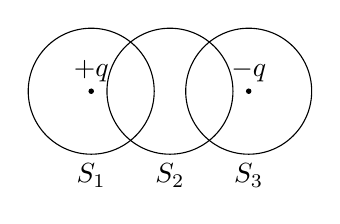
\begin{tikzpicture}
\draw (0,0) circle (0.8);
\draw (0,-0.8) node[below] {$S_2$};
\draw (-1,0) circle (0.8);
\fill (-1,0) node[above] {$+q$} circle (1pt);
\draw (-1,-0.8) node[below] {$S_1$};
\draw (1,0) circle (0.8);
\fill (1,0) node[above] {$-q$} circle (1pt);
\draw (1,-0.8) node[below] {$S_3$};
\end{tikzpicture}
图63.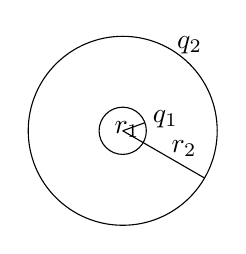
\begin{tikzpicture}[scale=0.3]
\draw (0,0) circle (1);
\draw (0,0) circle (4);
\draw (0,0) -- (20:1);
\draw (0,0) -- (330:4);
\draw (20:.2) node {$r_1$};
\draw (330:3) node[above] {$r_2$};
\draw (30:1) node[right] {$q_1$};
\draw (45:4) node[above] {$q_2$};
\end{tikzpicture}
图68.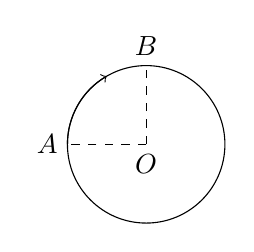
\begin{tikzpicture}
\draw (0,0) node[below] {$O$} circle (1);
\draw[dashed] (0,0) -- (90:1) node[above] {$B$};
\draw[dashed] (0,0) -- (180:1) node[left] {$A$};
\draw[->] (180:1) arc (180:120:1);
\end{tikzpicture}

63. 如图所示,两同心带电球面,内球面半径为$r_1=5$cm,带电荷$q_1=3\E{-8}$C;外球面半径为$r_2=20$cm,带电荷$q_2=-6\E{-8}$C.设无穷远处电势为零,则空间另一电势为零的球面半径$r=$\fbox{$10$cm}.

66. 把一个均匀带有电荷$+Q$的球形肥皂泡由半径$r_1$吹胀到$r_2$,则半径为$R$($r_1<R<r_2$)的球面上任意点的场强大小\fbox{$E$由$\frac{Q}{4\pi\eo R^2}$变为$0$},电势\fbox{$U$由$\frac{Q}{4\pi\eo R}$变为$\frac{Q}{4\pi\eo r_2}$}.

68. 在静电场中,一质子(带电荷$e=1.6\E{-19}$C)沿四分之一圆弧轨道从$A$点移到$B$点(如图),电场力做功$8.0\E{-15}$J.则当质子沿四分之三圆弧轨道从$B$点回到$A$点时,电场力做功$A=$\fbox{$-8.0\E{-15}$J}.设$A$点电势为零,则$B$点电势$U=$\fbox{$-5\E4$V}.


\subsubsection*{三. 计算题}

98. 如图所示,真空中一长为$L$的均匀带电细支杆,总电荷为$q$,试求在直杆延长线上距杆的一端距离为$d$的$P$点的电场强度.

\hfill
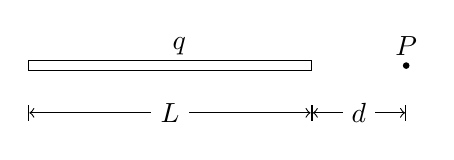
\begin{tikzpicture}[scale=1.2]
\draw (0,-0.05) rectangle (3,0.05);
\draw (1.6,0.2) node {$q$};
\draw[|<->|] (0,-0.5) -- (3,-0.5);
\draw (1.5,-0.5) node[fill=white] {$L$};
\fill (4,0) circle (1pt);
\draw (4,0) node[above] {$P$};
\draw[|<->|] (3,-0.5) -- (4,-0.5);
\draw (3.5,-0.5) node[fill=white] {$d$};
\end{tikzpicture}
\hfill
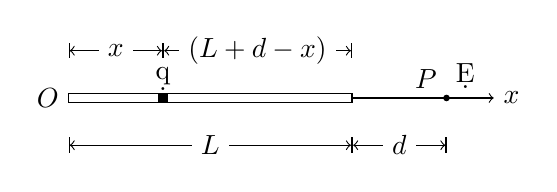
\begin{tikzpicture}[scale=1.2]
\draw (0,0) node[left] {$O$};
\draw (0,-0.05) rectangle (3,0.05);
\draw (1,0.2) node {$\d q$};
\draw[|<->|] (0,-0.5) -- (3,-0.5);
\draw (1.5,-0.5) node[fill=white] {$L$};
\fill (4,0) circle (1pt);
\draw (4,0) node[above left] {$P$};
\draw[|<->|] (3,-0.5) -- (4,-0.5);
\draw (3.5,-0.5) node[fill=white] {$d$};
\draw[|<->|] (0,0.5) -- (1,0.5);
\fill (0.95,-0.05) rectangle (1.05,0.05);
\draw (0.5,0.5) node[fill=white] {$x$};
\draw[|<->|] (1,0.5) -- (3,0.5);
\draw (2,0.5) node[fill=white] {$(L+d-x)$};
\draw[->] (3,0) -- (4.5,0) node[right] {$x$};
\draw (4.2,0) node[above] {$\d E$};
\end{tikzpicture}
\hfill

\SL{建立图示坐标系,带电直杆的电荷线密度为$\lambda=q/L$,
在$x$处取一电荷元$\d q=\lambda\delta x=q\d x/L$,
它在$P$点的元场强$\d E=\frac{\d q}{4\pi\eo (L+d-x)^2}=\frac{q\d x}{4\pi\eo L(L+d-x)^2}$.\\
因各元场强在$P$点的元场强均同向,所以可直接求和.\\
总场强$E=\frac{q}{4\pi\eo L}\int_0^L\frac{\d x}{(L+d-x)^2}=\frac{q}{4\pi\eo d(l+d)}$,
方向沿$x$轴,即杆的延长线方向.
}
99. 一个细玻璃棒被弯成半径为$R$的半圆形,沿其上半部分均匀分布有电荷$+Q$,沿其下半部分均匀分布有电荷$-Q$,如图所示.试求圆心$O$处的电场强度.

\hfill
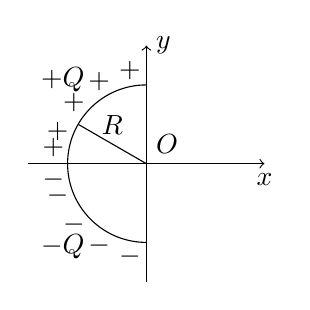
\begin{tikzpicture}
\draw[->] (-1.5,0) -- (1.5,0) node[below] {$x$};
\draw[->] (0,-1.5) -- (0,1.5) node[right] {$y$};
\draw (0,0) node[above right] {$O$};
\draw (90:1) arc (90:270:1);
\foreach \x in {100,120,140,160,170}
    \draw (\x:1.2) node {$+$};
\foreach \x in {190,200,220,240,260}
    \draw (\x:1.2) node {$-$};
\draw (0,0) -- (150:1);
\draw (150:0.5) node[above] {$R$};
\draw (135:1.5) node {$+Q$};
\draw (225:1.5) node {$-Q$};
\end{tikzpicture}
\hfill
\begin{tikzpicture}
\draw[->] (-1.5,0) -- (1.5,0) node[below] {$x$};
\draw[->] (0,-1.5) -- (0,1.5) node[right] {$y$};
\draw (0,0) node[above right] {$O$};
\draw (90:1) arc (90:270:1);
\foreach \x in {100,120,140,160,175}
    \draw (\x:1.2) node {$+$};
\foreach \x in {185,200,220,240,260}
    \draw (\x:1.2) node {$-$};
\draw (0,0) -- (230:1);
\draw (230:0.5) node[above] {$R$};
\draw (135:1.5) node {$\d q$};
% \draw (225:1.5) node {$\d q$};

\draw (0,0) -- (130:1);
\draw (90:0.2) arc (90:130:0.2);
\draw (110:0.4) node {$\theta$};
\draw (0,0) -- (145:1);
\draw (130:0.3) arc (130:145:0.3);
\draw (137.5:0.7) node {$\d\theta$};
\draw[->] (0,0) -- (310:1) node[below] {$\d\vec E$};
\draw (270:0.2) arc (270:310:0.2);
\draw (285:0.4) node {$\theta$};
\end{tikzpicture}
\hfill

\SL{把所有电荷都当作正电荷处理.
在$\theta$处取微小电荷$\d q=\lambda\d l=\frac{Q}{\frac{R}{2}\pi}\cdot R\d\theta=\frac{2Q\d\theta}{\pi}$.\\
它在$O$处产生场强$\d E=\frac{\d q}{4\pi\eo  R^2}=\frac{Q}{2\pi^2\eo  R^2}\d\theta$,
将$\d E$分解成两个分量:\\
$\d E_x=\d E\sin\theta=\frac{Q}{4\pi^2\eo  R^2}\sin\theta\d\theta$,
$\d E_y=-\d E\cos\theta=\frac{Q}{4\pi^2\eo  R^2}\cos\theta\d\theta$.\\
对各分量分别积分,考虑到一半是负电荷\\
$E_x=\frac{Q}{4\pi^2\eo  R^2}\left[\int_0^{\pi/2}\sin\theta\d\theta-\int_{\pi/2}^{\pi}\sin\theta\d\theta\right]=0$,\\
$E_y=\frac{-Q}{4\pi^2\eo  R^2}\left[\int_0^{\pi/2}\cos\theta\d\theta-\int_{\pi/2}^{\pi}\cos\theta\d\theta\right]=\frac{-Q}{\pi^2\eo  R^2}$.\\
所以$\vec E=E_x\vec\imath+E_y\vec\jmath=\frac{-Q}{\pi^2\eo  R^2}\vec\jmath$.
}
101. 半径为$R$的带电细圆环,其电荷线密度为$\lambda=\lambda_0\sin\phi$,式中$\lambda_0$为一常数,$\phi$为半径$R$与$x$轴所成的夹角,如图所示,试求环心$O$处的电场强度.

\hfill
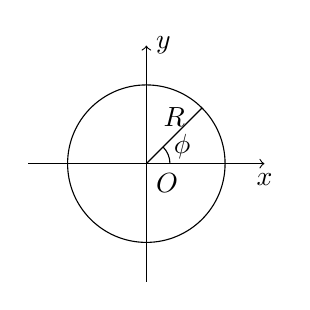
\begin{tikzpicture}
\draw[->] (-1.5,0) -- (1.5,0) node[below] {$x$};
\draw[->] (0,-1.5) -- (0,1.5) node[right] {$y$};
\draw (0,0) node[below right] {$O$};
\draw (0,0) circle (1);
\draw (0,0) -- (45:1);
\draw (45:0.5) node[above] {$R$};
\draw (0.3,0) arc (0:45:0.3);
\draw (25:0.5) node {$\phi$};
\end{tikzpicture}
\hfill
\begin{tikzpicture}
\draw[->] (-1.5,0) -- (1.5,0) node[below] {$x$};
\draw[->] (0,-1.5) -- (0,1.5) node[right] {$y$};
\draw (0,0) node[below right] {$O$};
\draw (0,0) circle (1);
\draw (0,0) -- (45:1);
\draw (45:0.5) node[above] {$R$};
\draw (0.3,0) arc (0:45:0.3);
\draw (25:0.5) node {$\phi$};
\draw[dashed] (0,0) -- (50:1);
\draw (47:1.4) node[above] {$\d q$};
\draw (45:0.5) arc (45:50:0.5);
\draw (44:1.2) node {$\d\phi$};
\draw[->,thick] (0,0) -- (-0.6,0) node[above] {$\d E_x$};
\draw[->,thick] (0,0) -- (0,-0.6) node[right] {$\d E_y$};
\draw[dashed] (-0.6,0) -- (-0.6,-0.6) node[below] {$\d E$};
\draw[dashed] (0,-0.6) -- (-0.6,-0.6);
\draw[->] (0,0) -- (-0.6,-0.6);
\draw (-0.3,0) arc (180:225:0.3);
\draw (200:0.5) node {$\phi$};
\end{tikzpicture}
\hfill

\SL{在任意角$\phi$处取微小电量$\d q=\lambda\d l$,\\
它在$O$点产生的场强为
$\d E=\frac{\lambda\d l}{4\pi\eo R^2}=\frac{\lambda_0\sin\phi\d\phi}{4\pi\eo R}$.\\
它沿$x,y$轴上的两个分量为
$\d E_x=-\d E\cos\phi$,
$\d E_y=-\d E\sin\phi$,\\
对各分量分别求和
$E_x=-\frac{\lambda_0}{4\pi\eo R}\int_0^{2\pi}\sin\phi\d(\sin\phi)\d\phi=0$,\pp
$E_y=-\frac{\lambda_0}{4\pi\eo R}\int_0^{2\pi}\sin^2\phi\d\phi=-\frac{\lambda_0}{4\eo R}$.
故$O$点的场强为$\vec E=E_y\vec\jmath=-\frac{\lambda_0}{4\eo R}\vec\jmath$.
}
102. 图中所示,$A,B$为真空中两个平行的“无限大”均匀带电平面,$A$面上电荷面密度$\sigma_A=-17.7\E{-8}\Cmm$,$B$面的电荷面密度$\sigma_B=35.4\E{-8}\Cmm$.试计算两平面之间和两平面外的电场强度.

\hfill
\begin{tikzpicture}[yscale=0.6]
\draw (0,0) -- (0,3);
\draw[dashed] (0,-1) -- (0,4);
\draw (1,0) -- (1,3);
\draw[dashed] (1,-1) -- (1,4);
\draw (0,3) node[above] {$\sigma_A$};
\draw (0,0) node[right] {$A$};
\draw (1,3) node[above] {$\sigma_B$};
\draw (1,0) node[right] {$B$};
\end{tikzpicture}
\hfill
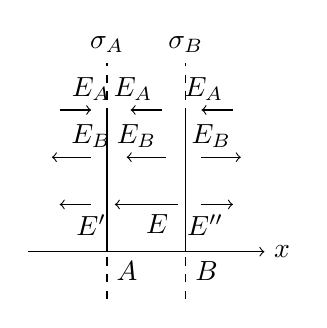
\begin{tikzpicture}[yscale=0.6]
\draw (0,0) -- (0,3);
\draw[dashed] (0,-1) -- (0,4);
\draw (1,0) -- (1,3);
\draw[dashed] (1,-1) -- (1,4);
\draw (0,4) node[above] {$\sigma_A$};
\draw (0,0) node[below right] {$A$};
\draw (1,4) node[above] {$\sigma_B$};
\draw (1,0) node[below right] {$B$};
\draw[->] (-1,0) -- (2,0) node[right] {$x$};
\draw[->] (-0.6,3) -- (-0.2,3) node[above] {$E_A$};
\draw[<-] (0.3,3) -- (0.7,3) node[above left] {$E_A$};
\draw[<-] (1.2,3) -- (1.6,3) node[above left] {$E_A$};
\draw[<-] (-0.7,2) -- (-0.2,2) node[above] {$E_B$};
\draw[<-] (0.25,2) -- (0.75,2) node[above left] {$E_B$};
\draw[->] (1.2,2) -- (1.7,2) node[above left] {$E_B$};
\draw[<-] (-0.6,1) -- (-0.2,1) node[below] {$E'$};
\draw[<-] (0.1,1) -- (0.9,1) node[below left] {$E$};
\draw[->] (1.2,1) -- (1.6,1) node[below left] {$E''$};
\end{tikzpicture}
\hfill

\SL{两带电平面各自产生的场强分别是\pp
$E_A=|\sigma_A|/(2\eo )$,方向如图示;
$E_B=\sigma_B/(2\eo )$,方向如图示.\\
建立坐标正向如图.
由叠加原理得:\\
两面间电场强度为$E=E_A+E_B=(|\sigma_A|+\sigma_B)/(2\eo )=3\E4\dw{N/C}$,方向沿$x$轴负方向;\\
两面外左侧$E'=E_A-E_B=(|\sigma_A|-\sigma_B)/(2\eo )=-1\E4\dw{N/C}$,方向沿$x$轴负方向;\\
两面外右侧$E''=E_B-E_A=1\E4\dw{N/C}$,方向沿$x$轴正方向.
}
103. 如图所示,一电荷面密度为$\sigma$的“无限大”平面,在距离平面$a$处的一点的场强大小的一半是由平面上的一个半径为$R$的圆面积范围内的电荷所产生的.试求该圆半径的大小.

\hfill
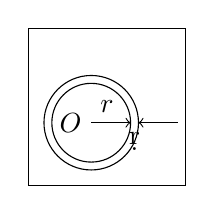
\begin{tikzpicture}
\draw (0,0) rectangle (2,2);
\draw (0.8,0.8) circle (0.5);
\draw (0.8,0.8) circle (0.6);
\draw (0.8,0.8) node[left] {$O$};
\draw[->] (0.8,0.8) -- (1.3,0.8);
\draw[->] (1.9,0.8) -- (1.4,0.8);
\draw (1.0,0.8) node[above] {$r$};
\draw (1.35,0.8) node[below] {$\d r$};
\end{tikzpicture}
\hfill

\SL{电荷面密度为$\sigma$的无限大均匀带电平面在任意点的场强大小为$E=\sigma/(2\eo)$.\\
以图中$O$点为圆心,取半径为$r\to r+\d r$的环形面积,其电量为$\d q=\sigma 2\pi r\d r$,\\
在它距离平面为$a$处的一点处产生的场强$\d E=\frac{\sigma ar\d r}{2\eo(a^2+r^2)^{\frac{3}{2}}}$.\\
则半径为$R$的圆面积内的电荷在该点的场强为$E=\frac{\sigma a}{2\eo}\int_0^R\frac{r\d r}{(a^2+r^2)^{\frac{3}{2}}}=\frac{\sigma}{2\eo}\left(1-\frac{a}{\sqrt{a^2+R^2}}\right)$.\\
由题意,令$E=\sigma/(4\eo)$,得到$R=\sqrt3 a$.
}
118. 图中所示为一$x$轴放置的长度为$l$的不均匀带电细棒,其电荷线密度为$\lambda=\lambda_0(x-a)$,$\lambda_0$为一常量.取无穷远处为电势零点,求坐标原点$O$处的电势.

\hfill
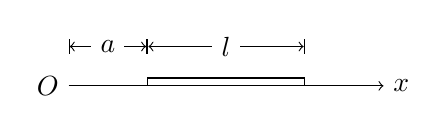
\begin{tikzpicture}
\draw[->] (0,0) node[left] {$O$} -- (4,0) node[right] {$x$};
\draw (1,0) rectangle (3,0.1);
\draw[|<->|] (0,0.5) -- (1,0.5);
\draw (0.5,0.5) node[fill=white] {$a$};
\draw[|<->|] (1,0.5) -- (3,0.5);
\draw (2,0.5) node[fill=white] {$l$};
\end{tikzpicture}
\hfill
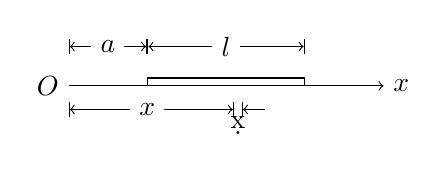
\begin{tikzpicture}
\draw[->] (0,0) node[left] {$O$} -- (4,0) node[right] {$x$};
\draw (1,0) rectangle (3,0.1);
\draw[|<->|] (0,0.5) -- (1,0.5);
\draw (0.5,0.5) node[fill=white] {$a$};
\draw[|<->|] (1,0.5) -- (3,0.5);
\draw (2,0.5) node[fill=white] {$l$};
\draw[|<->|] (0,-0.3) -- (2.1,-0.3);
\draw (1,-0.3) node[fill=white] {$x$};
\draw[->|] (2.5,-0.3) -- (2.2,-0.3);
\draw (2.15,-0.5) node {$\d x$};
\end{tikzpicture}
\hfill

\SL{分割带电细棒,任取线元$\d x$,其带电荷$\d q=\lambda_0(x-a)\d x$.\\
它在$O$点产生的元电势$\d U=\frac{\lambda_0(x-a)\d x}{4\pi\eo x}$.\\
$O$点总电势$U=\int\d U=\frac{\lambda_0}{4\pi\eo}\left(\int_0^{a+l}\d x-a\int_a^{a+l}\frac{\d x}{x}\right)=\frac{\lambda_0}{4\pi\eo}\left(l-a\ln\frac{a+l}{a}\right)$.
}
